% !TEX program = pdflatex
% Tri-fold brochure built on the `leaflet` class (landscape A4, 6 panels).
% leaflet numbers the panels 1..6: sheet front = panels 5 | 6 | 1 (back cover,
% flap, front cover), sheet back = panels 2 | 3 | 4 (the inside spread).
% Print double-sided (flip on the long edge) and fold along the dashed lines.
% All graphics are drawn with TikZ, so no external images are required.
\documentclass[a4paper,11pt,foldmark,notumble]{leaflet}

\usepackage[utf8]{inputenc}
\usepackage[T1]{fontenc}
\usepackage[default]{lato}
\usepackage[dvipsnames]{xcolor}
\usepackage{tikz}
\usetikzlibrary{calc,shapes.geometric,arrows.meta,positioning,decorations.pathmorphing,backgrounds}
\usepackage{enumitem}
\usepackage{booktabs}
\usepackage{microtype}
\usepackage[hidelinks]{hyperref}

%---------------------------------------------------------------------
% Palette and helpers
%---------------------------------------------------------------------
\definecolor{brand}{HTML}{0B4F6C}      % deep teal
\definecolor{brandlight}{HTML}{E3F2F7} % pale teal
\definecolor{accent}{HTML}{F4A259}     % warm orange
\definecolor{ink}{HTML}{2B2B2B}

\color{ink}
\setlength{\parindent}{0pt}
\setlength{\parskip}{0.55em}
\AddToBackground{1}{%
  \tikz[remember picture,overlay]
    \fill[brandlight] (current page.north west) rectangle
      ([yshift=-1.2cm]current page.north east);}
\CutLine*{1}\CutLine*{2}\CutLine*{3}\CutLine*{4}\CutLine*{5}\CutLine*{6}

% Section header: colored band with white caps text
\newcommand{\panelhead}[1]{%
  \begin{tikzpicture}
    \node[fill=brand, text=white, font=\large\bfseries, inner xsep=8pt, inner ysep=5pt,
          minimum width=\linewidth, align=left, text width=\linewidth-16pt] {#1};
  \end{tikzpicture}\par\vspace{0.3em}}

% Small subsection title in brand color
\newcommand{\subhead}[1]{{\color{brand}\bfseries #1}\par}

% Icon-like glyphs drawn with TikZ (no icon fonts needed)
\newcommand{\iconflask}{%
  \tikz[baseline=-0.4ex,scale=0.9]{
    \draw[brand, thick, rounded corners=0.5pt] (-0.1,0.35) -- (-0.1,0.05) -- (-0.3,-0.3) -- (0.3,-0.3) -- (0.1,0.05) -- (0.1,0.35);
    \fill[accent] (-0.22,-0.28) -- (0.22,-0.28) -- (0.1,-0.08) -- (-0.1,-0.08) -- cycle;
    \draw[brand, thick] (-0.17,0.35) -- (0.17,0.35);}}
\newcommand{\iconcode}{%
  \tikz[baseline=-0.4ex,scale=0.9]{
    \draw[brand, thick] (-0.3,0.15) -- (-0.4,0) -- (-0.3,-0.15);
    \draw[brand, thick] (0.3,0.15) -- (0.4,0) -- (0.3,-0.15);
    \draw[accent, thick] (0.1,0.25) -- (-0.1,-0.25);}}
\newcommand{\icongear}{%
  \tikz[baseline=-0.4ex,scale=0.9]{
    \fill[brand] (0,0) circle (0.22);
    \foreach \a in {0,45,...,315} \fill[brand, rotate=\a] (-0.06,0.18) rectangle (0.06,0.3);
    \fill[white] (0,0) circle (0.09);}}
\newcommand{\iconpin}{%
  \tikz[baseline=-0.4ex,scale=0.9]{
    \fill[brand] (0,0.1) circle (0.22);
    \fill[brand] (-0.19,0) -- (0,-0.35) -- (0.19,0) -- cycle;
    \fill[white] (0,0.12) circle (0.08);}}
\newcommand{\iconclock}{%
  \tikz[baseline=-0.4ex,scale=0.9]{
    \draw[brand, thick] (0,0) circle (0.26);
    \draw[brand, thick] (0,0) -- (0,0.17);
    \draw[accent, thick] (0,0) -- (0.14,-0.05);}}
\newcommand{\iconmail}{%
  \tikz[baseline=-0.4ex,scale=0.9]{
    \draw[brand, thick, fill=white] (-0.32,-0.2) rectangle (0.32,0.2);
    \draw[brand, thick] (-0.32,0.2) -- (0,-0.03) -- (0.32,0.2);}}

\begin{document}

%---------------------------------------------------------------------
% Panel 1: front cover (outside, right)
%---------------------------------------------------------------------
\begin{center}
\vspace*{0.4cm}
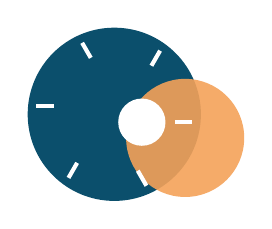
\begin{tikzpicture}
  % logo: overlapping circles + spark
  \fill[brand] (0,0) circle (1.1);
  \fill[accent, opacity=0.9] (0.9,-0.3) circle (0.75);
  \fill[white] (0.35,-0.1) circle (0.3);
  \foreach \a in {0,60,...,300}
    \draw[white, line width=1.5pt, rotate=\a] (0.35,-0.1) ++(0:0.42) -- ++(0:0.22);
  \node[white, font=\bfseries\Large, anchor=east] at (-0.2,0.35) {};
\end{tikzpicture}

\vspace{0.6cm}
{\fontsize{30}{34}\selectfont\bfseries\color{brand} Open Lab\par}
\vspace{0.1cm}
{\Large\color{accent}\bfseries Workshop Series 2026\par}

\vspace{0.8cm}

\begin{tikzpicture}
  \draw[brand, line width=1pt] (0,0) -- (5.5,0);
  \fill[accent] (2.75,0) circle (0.12);
\end{tikzpicture}

\vspace{0.6cm}
{\large Hands-on sessions in\\[2pt] science, making and code\par}

\vspace{1.0cm}

\begin{tikzpicture}[every node/.style={font=\small}]
  \node (a) {\iconflask};
  \node[right=0.9cm of a] (b) {\iconcode};
  \node[right=0.9cm of b] (c) {\icongear};
  \node[below=0.1cm of a] {Explore};
  \node[below=0.1cm of b] {Build};
  \node[below=0.1cm of c] {Share};
\end{tikzpicture}

\vfill
{\small One Saturday a month. Free. Everyone welcome.\par}
\vspace{0.4cm}
\end{center}

\newpage

%---------------------------------------------------------------------
% Panel 2: inside left
%---------------------------------------------------------------------
\panelhead{What is Open Lab?}

Open Lab is a community workshop series where curious people learn by doing.
Each session is a full day in a well-equipped lab, guided by volunteers who
work in research, industry and the arts.

You do not need a degree, a laptop or prior experience: we provide the
equipment, the materials and a printed guide to take home.

\subhead{Who it is for}
\begin{itemize}[leftmargin=1.2em, itemsep=0.1em]
  \item Students who want to try a field before committing to it.
  \item Professionals picking up a new tool for their work.
  \item Teachers looking for classroom-ready activities.
  \item Anyone who enjoys taking things apart to see how they work.
\end{itemize}

\subhead{Our numbers so far}
\begin{center}
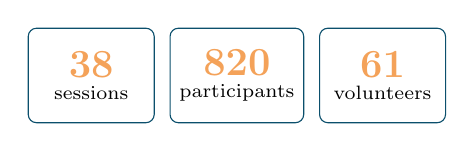
\begin{tikzpicture}[x=1cm, y=1cm, font=\scriptsize]
  \foreach \v/\l/\i in {38/sessions/0, 820/participants/1, 61/volunteers/2} {
    \node[draw=brand, rounded corners=3pt, minimum width=1.6cm, minimum height=1.2cm,
          align=center, fill=white] at (\i*1.85,0)
          {{\color{accent}\Large\bfseries\v}\\\l};
  }
\end{tikzpicture}
\end{center}

\newpage

%---------------------------------------------------------------------
% Panel 3: inside centre
%---------------------------------------------------------------------
\panelhead{How a Session Works}

\begin{center}
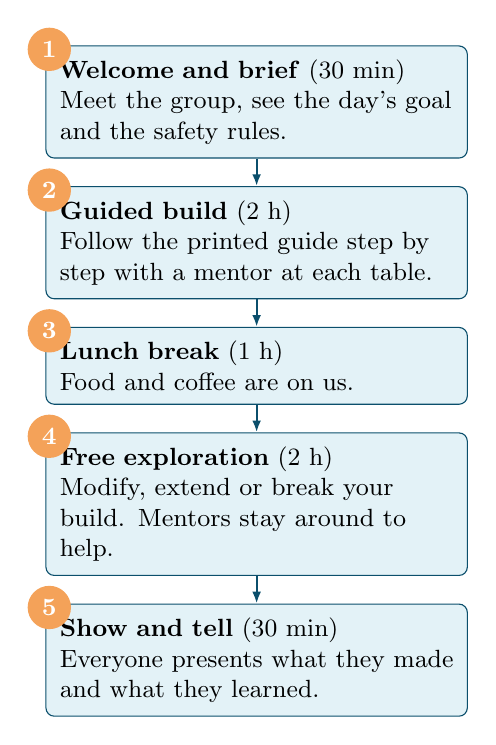
\begin{tikzpicture}[
    node distance=0.35cm,
    stepbox/.style={draw=brand, fill=brandlight, rounded corners=3pt, text width=5.0cm,
                 align=left, inner sep=5pt, font=\small},
    num/.style={circle, fill=accent, text=white, font=\bfseries\small, minimum size=5.5mm, inner sep=0pt},
  ]
  \node[stepbox] (s1) {\textbf{Welcome and brief} (30 min)\\ Meet the group, see the day's goal and the safety rules.};
  \node[stepbox, below=of s1] (s2) {\textbf{Guided build} (2 h)\\ Follow the printed guide step by step with a mentor at each table.};
  \node[stepbox, below=of s2] (s3) {\textbf{Lunch break} (1 h)\\ Food and coffee are on us.};
  \node[stepbox, below=of s3] (s4) {\textbf{Free exploration} (2 h)\\ Modify, extend or break your build. Mentors stay around to help.};
  \node[stepbox, below=of s4] (s5) {\textbf{Show and tell} (30 min)\\ Everyone presents what they made and what they learned.};
  \foreach \n/\i in {s1/1, s2/2, s3/3, s4/4, s5/5}
    \node[num] at ($(\n.north west)+(0.05,-0.05)$) {\i};
  \foreach \a/\b in {s1/s2, s2/s3, s3/s4, s4/s5}
    \draw[-{Latex[length=1.5mm]}, brand, thick] (\a.south) -- (\b.north);
\end{tikzpicture}
\end{center}

\subhead{What to bring}
Just yourself. If you have a notebook or a favourite tool you want to use, bring it along.

\newpage

%---------------------------------------------------------------------
% Panel 4: inside right
%---------------------------------------------------------------------
\panelhead{Featured Workshops}

\subhead{\iconflask\ Open Data Night}
Turn a public dataset into an interactive dashboard in one afternoon. We
cover cleaning, charting and telling an honest story with numbers.

\subhead{\iconcode\ Typesetting with \LaTeX{}}
Write and compile a short paper with figures, tables and references. Leave
with a template you can reuse for your thesis or report.

\subhead{\icongear\ Build Your Own Synthesiser}
Solder a small analogue synth, learn how oscillators and filters shape
sound, and jam with the group at the end of the day.

\vspace{0.3em}

\begin{tikzpicture}
  \node[fill=brand, text=white, rounded corners=4pt, inner sep=8pt,
        text width=\linewidth-16pt, align=left] {%
    {\bfseries\large Register}\\[3pt]
    Scan nothing, click nothing: just send an email with your name and the
    session you want to join to\\
    {\bfseries hello@openlab.example}\\[3pt]
    {\small We confirm within two working days.}};
\end{tikzpicture}

\vfill
{\small\color{gray} Workshops are held in Spanish and English. Materials are
provided; participants under 16 must be accompanied by an adult.\par}

\newpage

%---------------------------------------------------------------------
% Panel 5: back cover (outside, left)
%---------------------------------------------------------------------
\panelhead{Find Us}

\begin{itemize}[leftmargin=2em, itemsep=0.6em, labelsep=0.6em]
  \item[\iconpin] \textbf{Open Lab, Building C}\\
    Campus Innovation Hub\\
    Av.\ Universitaria 1801, Lima
  \item[\iconclock] \textbf{Second Saturday} of every month\\
    10:00 -- 16:00, lunch included
  \item[\iconmail] hello@openlab.example\\
    openlab.example/workshops
\end{itemize}

\subhead{How to get there}
\begin{center}
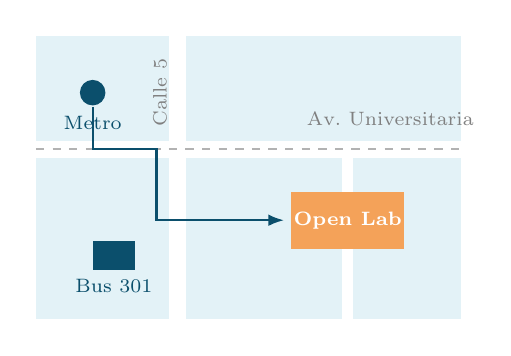
\begin{tikzpicture}[scale=0.9, every node/.style={font=\scriptsize}]
  % simplified map
  \fill[brandlight] (-3,-2) rectangle (3,2);
  \draw[white, line width=6pt] (-3,0.4) -- (3,0.4);
  \draw[white, line width=6pt] (-1,-2) -- (-1,2);
  \draw[white, line width=4pt] (1.4,-2) -- (1.4,0.4);
  \draw[gray!60, line width=0.8pt, dashed] (-3,0.4) -- (3,0.4);
  \node[above, gray] at (2,0.6) {Av.\ Universitaria};
  \node[rotate=90, gray] at (-1.25,1.2) {Calle 5};
  \fill[accent] (0.6,-1.0) rectangle (2.2,-0.2);
  \node[white, font=\scriptsize\bfseries] at (1.4,-0.6) {Open Lab};
  \fill[brand] (-2.2,1.2) circle (0.18);
  \node[below, brand] at (-2.2,1.0) {Metro};
  \fill[brand] (-2.2,-1.3) rectangle (-1.6,-0.9);
  \node[below, brand] at (-1.9,-1.3) {Bus 301};
  \draw[-{Latex[length=2mm]}, brand, thick] (-2.2,1.0) -- (-2.2,0.4) -- (-1.3,0.4) -- (-1.3,-0.6) -- (0.5,-0.6);
\end{tikzpicture}
\end{center}

\vfill
\subhead{Partners}
The workshop series is hosted by the Open Lab community and supported by the
Example University Library, the Lima Makers Collective and local volunteers.

{\small\color{gray} Open Lab is a fictional organisation used to demonstrate this template.}

\newpage

%---------------------------------------------------------------------
% Panel 6: flap (outside, centre; folds in behind the cover)
%---------------------------------------------------------------------
\panelhead{2026 Season at a Glance}

\subhead{Spring}
\begin{tabular}{@{}l p{4.4cm}@{}}
  \toprule
  Mar 14 & Open Data Night: from CSV to dashboard \\
  Apr 11 & Build a weather station with a microcontroller \\
  May 9  & Typesetting your first paper with \LaTeX{} \\
  \bottomrule
\end{tabular}

\subhead{Summer}
\begin{tabular}{@{}l p{4.4cm}@{}}
  \toprule
  Jun 13 & 3D printing: design, slice, print \\
  Jul 11 & Intro to machine learning with Python \\
  Aug 8  & Repair Caf\'e: fix it, don't toss it \\
  \bottomrule
\end{tabular}

\subhead{Autumn}
\begin{tabular}{@{}l p{4.4cm}@{}}
  \toprule
  Sep 12 & Reproducible research with containers \\
  Oct 10 & Build your own synthesiser \\
  Nov 14 & Showcase night and community awards \\
  \bottomrule
\end{tabular}

\vfill

\begin{tikzpicture}
  \node[draw=accent, line width=1.2pt, rounded corners=4pt, inner sep=7pt,
        text width=\linewidth-16pt, align=center, font=\small] {%
    \textbf{All sessions are free.}\\
    Seats are limited to 24 people, so please register in advance.};
\end{tikzpicture}

\end{document}
